\documentclass[journal=jacsat,manuscript=article]{achemso}
% \linespread{1.5}
\usepackage{amssymb,amsmath,graphics,epsfig}
% \usepackage{amsmath}
\usepackage[font=small,labelfont=bf]{caption}
\usepackage{multirow}
\usepackage{xcolor}
\usepackage{siunitx}
\usepackage{float}
\usepackage{upgreek}
\usepackage{soul}
\setkeys{acs}{super = true}
\setcitestyle{super,open={},close={}}
\def\citenumfont{}

% \usepackage[version=3]{mhchem} 
\usepackage{color}
\newcommand{\eqnref}[1]{Eqn.~\plainref{#1}}
\newcommand{\figref}[1]{Fig.~\plainref{#1}}
\newcommand{\tabref}[1]{Table~\plainref{#1}}

\title{Making Soup: Preparing and Validating Molecular Simulations of the Bacterial Cytoplasm}


\author{Leandro Oliveira Bortot}
\affiliation{Laboratory of Biological Physics, School of Pharmaceutical Sciences of Ribeir{\~a}o Preto, University of S{\~a}o Paulo, Ribeir{\~a}o Preto, Brazil}
\altaffiliation{These authors contributed equally to this work}

\author{Zahedeh Bashardanesh}
\affiliation{Science for Life Laboratory, Department of Cell and Molecular Biology. Uppsala University, SE-751 05 Uppsala, Sweden}
\altaffiliation{These authors contributed equally to this work}

\author{David van der Spoel}
\affiliation{Science for Life Laboratory, Department of Cell and Molecular Biology. Uppsala University, SE-751 05 Uppsala, Sweden}
\email{david.vanderspoel@icm.uu.se}


\begin{document}

\maketitle

\begin{abstract}
%For Nature, the abstract is really an introductory paragraph set
%in bold type.  This paragraph must be ``fully referenced'' and
%less than 180 words for Letters.  This is the thing that is
%supposed to be aimed at people from other disciplines and is
%arguably the most important part to getting your paper past the
%editors.  End this paragraph with a sentence like ``Here we
%show...'' or something similar.

 
\end{abstract}
\section*{Introduction}


%Biomolecules move and function in an environment densely packed with high concentrations of macromolecules. The presence of macromolecules leads to steric effect due to excluded volume effect and intermolecular attrative/repulsive forces due to distributed charges on the surface of macromolecules.

The intracellular microenvironment is markedly different from the \textit{in vitro} simplification from which most of our current knowledge about the biochemical and biophysical behavior of macromolecules was derived~\cite{Feig2017a}. Instead of simple and diluted, the \textit{in vivo} microenvironment is highly heterogeneous and concentrated, leading to spatial constrains that directly affects biological activities~\citep{ostrowska2019}. Macromolecular crowding directly influences the stability of macromolecules. There is an equilibrium between stabilization of their native structure due to the entropic component given by the excluded volume effect~\cite{cheung2005} and destabilizationg due to enthalpic component given by unspecific interactions with the crowders~\cite{Feig2011,miklos2011,Wang2012b}. Additionally, crowding affects the structure and dynamics of water around proteins, which has an indirect but important effect in their biological activities~\cite{Harada2012a,king2013}.

While the structure and dynamics of biomolecules is well characterized \textit{in vitro}, the understanding of the influences of crowded environments for the \textit{in vivo} are still evolving.  Techniques such as nuclear magnetic resonance~\cite{reckel2007,pielak2008} and fluorescence spectroscopy~\cite{ignatova2004,xie2008,English2011} are among the most relevant to the field due to their ability to probe cells in a non destructive way. Another essential class of methods come from computational modeling and simulation. By extrapolating the advances in computational power in the last decades to the future, it has been estimated that the atomistic simulation of an entire \textit{Escherichia coli} bacterium for \SI{1}{\nano\second} will be possible in 15 years from now~\cite{vanGunsteren2006a}.

As the available computational power increases, models become increasingly complex and are better representations of reality. The most simple class of computational models apply Brownian Dynamics calculations to probe macromolecules immersed in a solution of crowders that are treated as hard spheres with varying radius to represent different types of molecules~\cite{Ando2010}. These models usually use an implicit representation of the solvent~\cite{Mcguffee2010}. More recently, all-atom explicit solvent molecular dynamics simulations have been employed on crowded systems composed of several copies of one or a few macromolecules~\cite{Wang2017c}. However, these models doesn't reflect the true heterogeneity of biologically relevant crowded environments such as the cytoplasm. This was addressed by the development of a detailed model for the cytoplasm of the bacterium \textit{Mycoplasma genitalium} containing 103 million atoms~\cite{Feig2015}. This model, as well as a smaller version with 13 million atoms, was submitted to molecular dynamics simulations~\cite{Yu2016a}. Despite the size of these systems, the simulation times were too short, \SI{20}{\nano\second} for the complete model and \SI{140}{\nano\second} for the smaller version, to accurately characterize the effects of the slow diffusion of its constituents.

In this work we report an all-atom model of the cytoplasm of \textit{Escherichia coli} that was built to reflect the real biological system. We discuss the difficulties that arise when building such system and provide a set of Python scripts and files that anyone can use to build its own crowded systems with custom parameters and elements. Additionally, we performed long molecular dynamics simulations of our cytoplasm model, reaching \SI{3}{\micro\second} of total simulation time. This work is the first to explore the structural dynamics of an all-atom explicit solvent cytoplasm model with microsecond scale molecular dynamics simulations.



\section*{Materials and Methods}


\subsection*{Initial structures}
The proteins and tRNA were downloaded from Protein Data Bank (PDB). We looked for the proteins structures that were either from or expressed in {\em E-coli}. In case of 1U22 (MetE) and 2EIP (Ppa) we used a loop-closure modeling tool based on Random Coordinate Descent (RCD) method~\cite{Chys2013} to correct the information for missing residues. The four metabolites were parametrized using GAFF and Antechamber. 

\subsection*{Molecular Dynamics Simulation}

 
{\bf General Simulation Setup: }The proteins were simulated at 30\% biomolecular mass fraction in  a physiological salt concentration (0.15M NaCl). For all simulations, Amber99SB-ws force field was used~\cite{Best2014a} in combination with the TIP4P/2005 water model~\cite{Abascal2005b}. Electrostatic interactions were treated using the particle mesh Ewald algorithm~\cite{Essmann1995a}. All chemical bonds were constrained at their equilibrium length using the LINCS algorithm~\cite{Hess2008b} allowing an integration time step of 2 fs. Temperature was controlled at 310 K using the v-rescale algorithm~\cite{Bussi2007a} and a coupling time of 0.5 ps. The pressure was controlled at 1 bar using the Parrinello-Rahman algorithm~\cite{Parrinello1981a} with a time constant of 10 ps.  


For error analysis, each simulations were repeated three times with independent starting velocities.

All simulations were performed with Gromacs 2018. Single simulations were started from crystal conformations. The cytoplasm simulations starting conformation were taken from the equilibrated conformation of each single simulation.

{\bf Single Simulation Setup: } Each component was simulated with the same parameter as the cytoplasm for $200 ns$.

\subsection*{Analysis}
Before any analysis the periodic boundary condition (pbc) artifacts have been removed. We used GROMACS tools to do the analysis. For single component simulations, first the components were made whole and jump removed and then all the atom were put inside the compact box. The same treatment were applied to the cytoplasm simulations. Additionally, each component's trajectory were extracted and fitted by rotation and translation for later rotational correlation time analysis. 


A Mean Square Displacement (MSD) analysis was used to calculate the translational diffusion coefficient~\cite{Allen1987a}. The diffusion coefficients were extracted by a linear fit to MSD analysis by averaging blocks with a length of $10 \,ns$. In principle diffusion coefficient needs to be corrected for finite size effects~\cite{Yeh2004} but due to relatively large simulation boxes this correction is negligible.




\section*{Results}

\subsection{Cytoplasm model}
In this section we describe the rationale behind the composition of our model, which has five fractions: protein, RNA, metabolites, water and ions. We highlight that we didn't add lipids and DNA to our model because we are considering only elements that are free to diffuse through the cytosol. We gathered data from several sources in order to build a computational model that is representative of the cytoplasm of {\em Escheria coli}~\cite{Dong1996,Bennett2009,Link1997,Mcguffee2010}.

\subsubsection{Protein fraction}
We selected a group of eight proteins that account for 50\% of the abundance of non-ribosomal proteins in the cytoplasm of {\em Escherichia coli} \cite{Link1997}. The two most abundant proteins, TufA and MetE, account for about 20\% and 12\% of the total protein abundance in {\em E. coli}, respectively, while the other six proteins contribute with less than 5\% each (Table~\ref{tbl:protein_fraction}). Their crystallographic structures were used to insert them in the cytoplasm model. The number of copies of each protein in the model was calculated as the rounded up fold increase in their abundance when compared to the least abundant protein, which was set to have the copy number of 1. Then, this number was divided by the oligomeric state of each protein. This was done because the original oligomeric state for each protein was kept as reported in their crystallographic structure.

\begin{table}[H]
\centering
\begin{tabular}{ l c c c}
\hline
\multirow{2}{*}{Protein} & 	\multicolumn{2}{c}{Fraction [\%]} & \multirow{2}{*}{Oligomeric State}\\
& Absolute & Cumulative \\ 
\hline
TufA & 19.7 & 19.7 & 2-mer \\
MetE & 11.6 & 31.4 & 1-mer \\
IcdA & 4.7  & 36.1 & 2-mer \\
AhpC & 4.1  & 40.2 & 10-mer \\
CspC & 4.0  & 44.2 & 1-mer \\
Ppa  & 2.9  & 47.0 & 6-mer \\
GapA & 2.1  & 49.1 & 4-mer \\
Eno  & 1.9  & 51.1 & 2-mer \\
\hline
\end{tabular}
\caption{Absolute and cumulative fraction of the total abundance of non-ribosomal proteins in the cytosol of {\em E. coli} K12 to which each protein that was selected to compose our cytoplasm model corresponds to.}
\label{tbl:protein_fraction}
\end{table}


\subsubsection{RNA fraction}
Transporter RNAs (tRNAs) account for 74\% of the dry weight of non-ribosomal RNAs~\cite{phillips2012}. Thus, we chose to model the RNA presence in the cytoplasm with tRNA molecules. Specifically, we considered the tRNA(Phe) molecule as a representative of tRNAs due to the availability of a recent crystallographic structure~\cite{Byrne2015}.
The protein and RNA content of the total dry weight of \textit{E.coli} is 55\% and 2.9\%, respectively~\cite{phillips2012}. That is, the total RNA weight corresponds to 5\% of the total protein weight. This protein/RNA weight ratio was used to calculate the correct number of tRNA(Phe) molecules that were added to the cytoplasm model \tabref{tbl:soup_components}.

\subsubsection{Metabolites fraction}
We considered the most abundant molecules of each metabolite class as representatives, i.e. Glutamate for amino acids, ATP for nucleotides, FBP for central carbon intermediates and Glutathione redox cofactors~\cite{Bennett2009}. The total number of molecules was calculated considering data showing that the number of metabolite molecules in the cytoplasm of \textit{E. coli} is about 42.86 times higher than the number of proteins~\cite{Bennett2009}. The copy number for each molecule was calculated from the ratios between their experimentally observed concentration in {\em E. coli}~\cite{Bennett2009}.

\subsubsection{Water fraction}
The number of water molecules was calculated according to the desired biomolecular concentration, which is a parameter of the cytoplasm model. This number ranges from 300 to 400 $mg/ml$ in biological systems such as \textit{E. coli} cytoplasm~\cite{Zimmerman1991,Ellis2003a}. In our case, we choose the biomolecular concentration of 30\%, that is, the number of molecules necessary to reach a ratio of total biomolecular mass to water mass of 30\% was inserted into the cytoplasm model.

\subsubsection{Inorganic ions fraction}
Finally, Mg\textsuperscript{2+} was used as counter-ions for tRNA and ATP. K$^{+}$ and Cl$^{-}$ were added to neutralize the charges of the simulation box and to reach the ionic strength of 0.150 mol/L by substitution of randomly selected water molecules.



\begin{table}
\centering
\begin{tabular}{lcc}
\hline
Class & Name (PDB ID) & Number\\
\hline
Protein & TufA (1DG1~\cite{Abel1996}) & 6\\
  & MetE (1U22~\cite{Ferrer2004}) & 7\\
  & IcdA (1P8F~\cite{Mesecar2000}) & 2\\
  & AhpC (1YEP~\cite{Parsonage2005}) & 1\\
  & CspC (1MJC~\cite{Schindelin1994}) & 3\\
  & Ppa (2EIP~\cite{Kankare1996}) & 1\\
  & GapA (1S7C~\cite{ShinXXX}) & 1\\
  & Eno (1E9I~\cite{Kuhnel2001}) & 1\\
\hline
RNA & tRNA$^{\text{Phe}}$ (4YCO~\cite{Byrne2015}) & 5\\
\hline
Metabolite & GLU & 1436\\
  & ATP & 144\\
  & FBP & 225\\
  & GSH & 255\\
\hline
Solvent & Water & 306221\\
\hline
Inorganic Ion & K$^{+}$ & 4602\\
  & Mg$^{2+}$ & 400\\
  & Cl$^{-}$ & 1320\\
\hline
\end{tabular}
\caption{Number of copies for each component of the cytoplasm model built at the biomolecular fraction of 30\%}
\label{tbl:soup_components}
\end{table}



\subsection{Building the simulation box}
All components can be put in the same simulation box by inserting each of them in random orientations in a cubic box of side $L$ that is initially empty. However, that is not a trivial process. We need to use a box size that is big enough to allow the random insertions to succeed without structural overlapping and without creating artificial interactions between the elements by placing them too close from each other. On the other hand, as the box gets bigger, it gets harder to equilibrate the system because the empty space between the components will induce the barostat to reduce the box volume quickly during the simulation.

We devised an iterative process that solves both problems simultaneously. We start with a box size $L$ that is too small to allow all components to fit in the box by random insertion. In our case, we started with $L = 30$ nm. Then, we allow 100 insertion trials for each element. If all trials fail for any of them, we start the whole process again with an empty cubic box that is larger by a step size $dL$ of 1 nm. We repeat this process until all insertions succeed. In our case, all insertions succeeded after increasing $L$ to 35 nm. Additionally, instead of adding only the protein, tRNA or metabolite molecules in the empty box in each trial, we actually add a droplet of water and counter ions in which the molecule of interest is embedded. Such droplets are taken from molecular dynamics simulations in which each component was previously equilibrated. The benefits of using such droplets are threefold: \textit{i.} it acts as natural protecting layer that prevents artificial contacts between the components that could be created due to the random insertions. \textit{ii.} it is a natural way to place water molecules and counter-ions in the simulation box around each component. \textit{iii.} the components are already pre-equilibrated, which will help us to perform the equilibration of the whole cytoplasm model.

In order to do this, the droplets around each component are also constructed iteratively. The number of water molecules that we must place in the simulation box is known from the desired biomolecular fraction, which is a parameter of the model, and the total biomolecular mass of the system. However, we don't know the thickness of the water layer around each component, $l$, that accounts for such amount of water molecules. Since $l$ depends on a series of factors such as the shape, size and abundance of each element, we define it iteratively. We start by taking a droplet of thickness $l$ = 3 \r{A} around all elements and counting the number of water molecules that we would add to the box with such droplets. If it is smaller than the number we need, $l$ is increased by $dl$ = 1 \r{A}. If it is larger, we reduce the droplet thickness by $dl$, reduce $dl$ by 10 times and then increase $l$ with the new smaller $dl$. We can carry this process until an arbitrary precision cutoff, such as 5\%, is satisfied.


After all droplets are successfully inserted in a simulation box by the iterative process described above, we proceed to add ions to neutralize the net charge of the system and to reach the desired ionic strength. Then, we perform energy minimization and a short simulation step of 500ps in which all molecules of the box are free to move. In this step the box shrinks to its optimum size. In our case, the simulation box shrank from the initial box size of 35 nm to 22.9 nm, which correspond to a volume change from 42875 nm\textsuperscript{3} to 12009 nm\textsuperscript{3}. From this point, the system is ready to be submitted to the default simulation steps such as thermalization and production run (please check the materials section for details about the parameters we used).

\begin{figure}[H]
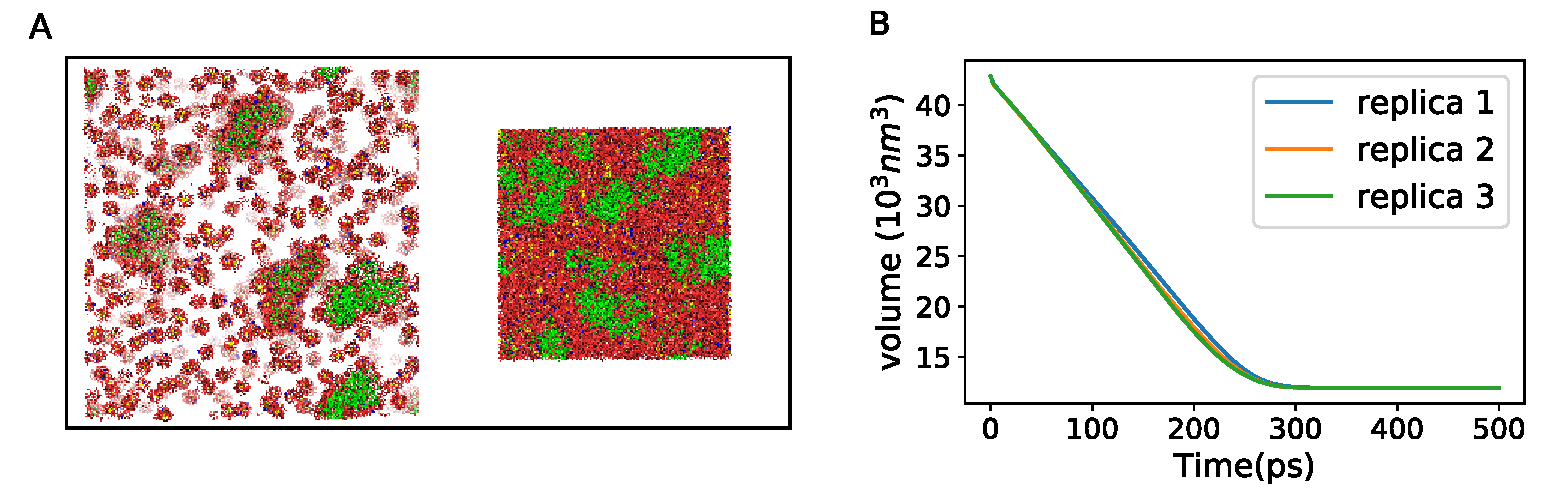
\includegraphics[scale=0.5]{shrinking.pdf} 
\caption{A) The volume of the box with length size of $L=35 \,\, nm$ reduces during the energy minimization in the first $300 \,\, ps$ B) The density of the same box increases within the first $300\,\, ps$. The repeated experiments are shown in different colors. }
\end{figure}



Python scripts and all topology and structure files necessary to enable any researcher to build its own cytoplasm models are publicly available at github.com/dspoel/soup. Such models can be used as tools that answer many research questions about the effects of crowding on specific systems of interest. With the files we are providing it is possible, for example, to add a probe protein to investigate the effect of crowding on it, to add new macromolecular or small crowders, verify the effects of different temperatures and change the biomolecular concentration to increase or decrease the intensity of the crowding effect.











\subsection{Effects of macromolecular crowding}

In order to investigate the effects of crowding in the \textit{E. coli} cytoplasm model on the structural integrity and dynamics of its elements, we constructed three completely independent cytoplasm models that have different orientations for each of its elements. We submitted these systems, each composed of more than 1.5 million atoms, to molecular dynamics simulations of \SI{1}{\micro\second}. We also performed \SI{200}{\nano\second} molecular dynamics simulations for each isolated element (proteins and tRNA) in order to represent the non-crowded, i.e. dilute environment (please check the materials section for details about the parameters).



% -------------------- TRANSLATIONAL DIFFUSION --------------------

\subsubsection{Translational diffusion}

Under crowded conditions, molecules are constrained to a smaller volume due to collisions with the other components of the crowded environment. The extent of this effect is evident when we compare the translational diffusion constant of each component in the cytoplasm model, $D_{cyto}$, and in a dilute system, $D_{dil}$ (Fig.~\ref{fig:translational_diffusion}A). The ratio of these quantities is independent of the protein size and is always close to 0.13 (Fig.~\ref{fig:translational_diffusion}B). However, the effect of crowding on the translational diffusion of tRNA is two times larger. Its $D_{cyto}/D_{dil}$ is 0.07, indicating that its movement is specially constrained in the crowded environment (Fig.~\ref{fig:translational_diffusion}B, crowder with 25 kDa).

\begin{figure}[H]
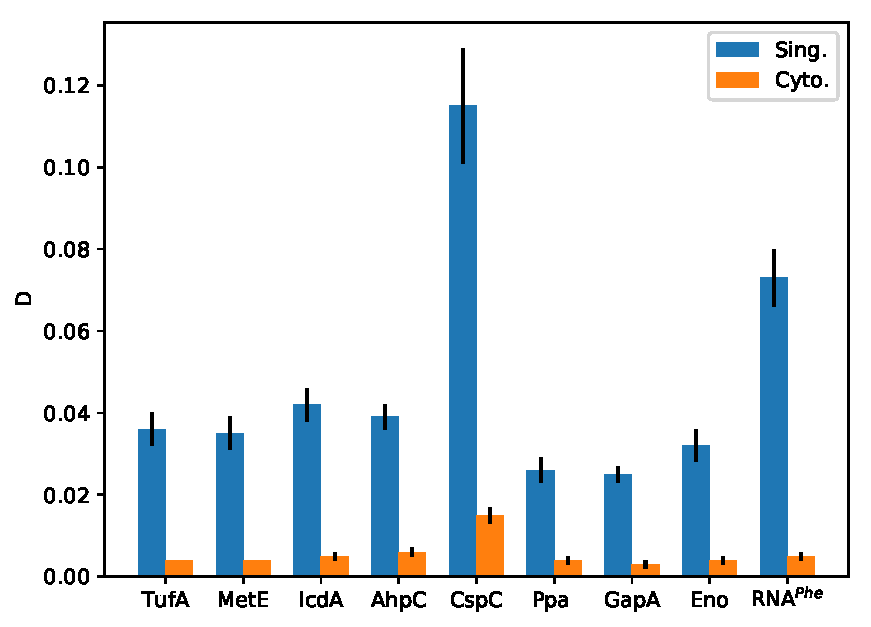
\includegraphics[scale=0.5]{msd.pdf}
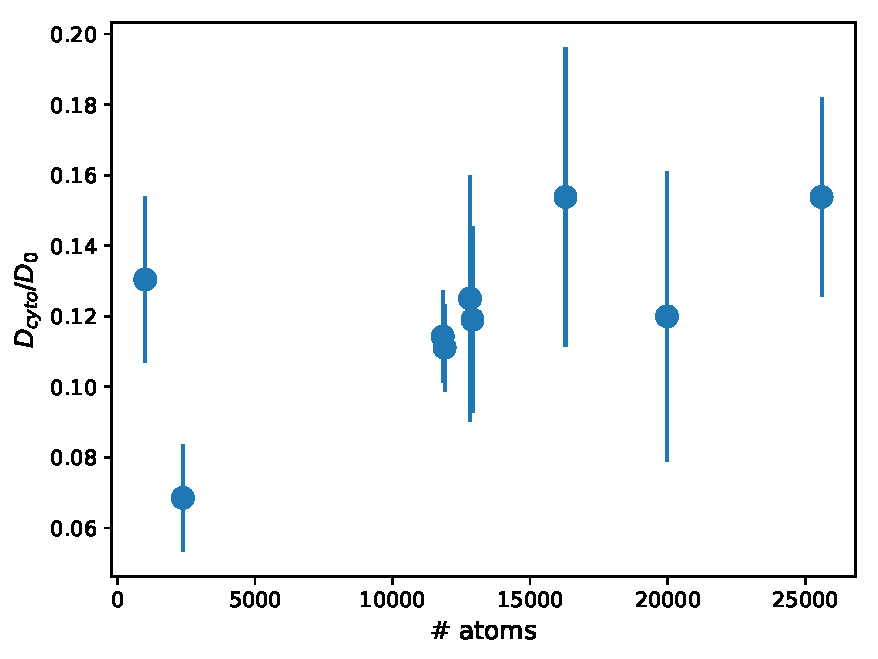
\includegraphics[scale=0.5]{diff_cyto_over_singles.pdf}
\caption{A) Diffusion coefficient of crowders from single molecule simulations (blue bars) and cytoplasm simulations (orange bars). B) The ratio between diffusion coefficient obtained from cytoplasm to single molecule simulations. The crowders are sorted according to their sizes on the x-axis.}
\label{fig:translational_diffusion}
\end{figure}

% \colorbox{green!50}{ Are we going to calculate and discuss rotational diffusion? No, not now at least.}









% -------------------- tRNA IS AN OUTLIER DUE TO AGGREGATION --------------------

\subsubsection{tRNA is aggregating}
After inspecting the trajectories of the cytoplasm models, we found that the reason why the translational diffusion constant for tRNA was reduced to a greater extent than for the other components of the cytoplasm model is that it is forming aggregates with Mg$^{2+}$, ATP and FBP (Fig.~\ref{fig:tRNA_aggregation}). Thus, in the next sections we will ignore the tRNA molecules in the analyses about the structural integrity of the crowders. Additionally, in the last section we will further investigate such aggregation and we will show a way to prevent it.

\begin{figure}[H]
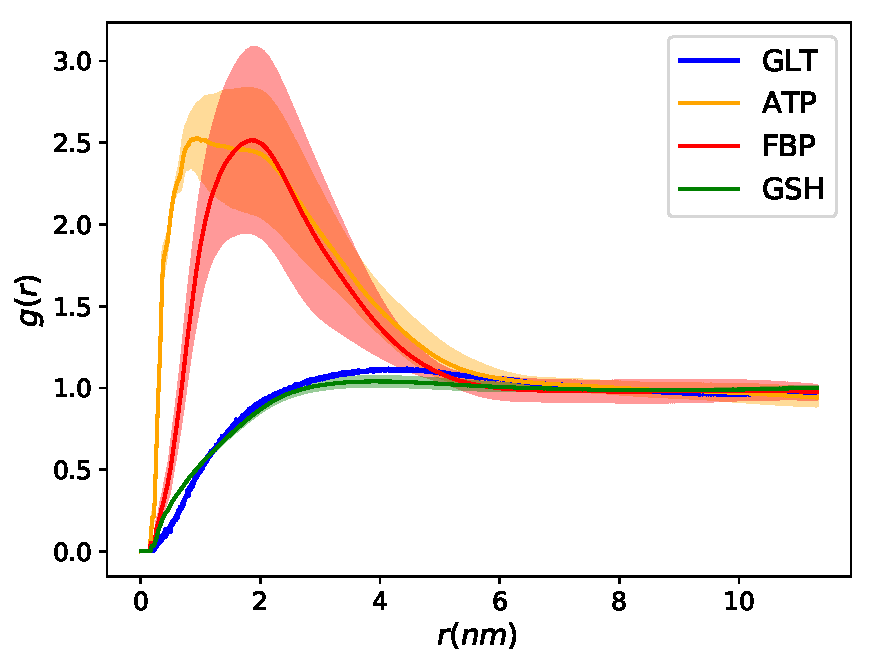
\includegraphics[scale=0.5]{rdf_RNA_metabolites.pdf}
\caption{Radial distribution function showing the probability of finding metabolites or Magnesium cations around tRNA molecules in the cytoplasm model.}
\label{fig:tRNA_aggregation}
\end{figure}



% -------------------- STRUCTURAL INTEGRITY OF SINGLE CHAINS --------------------

\subsubsection{Structural integrity}
The structure of the individual chains of the crowders that were used in our cytoplasm model were not affected to a great extent by the crowded environment. %\st{The solvent accessible surface area (SASA) value for all crowders in the cytoplasm model is within 5\% of its value under the dilute condition.} 
The root mean square deviation (RMSD) considering only their C$\upalpha$ atoms show that crowders remain intacts under crowded condition, except for TufA, MetE and IcdA, which have RMSD values 105, 25 and 33\% higher in the crowded environment than in the dilute condition. Visual inspection of their trajectories showed that there is partial unfolding of their N- or C-terminal residues. 
\begin{figure}[H]
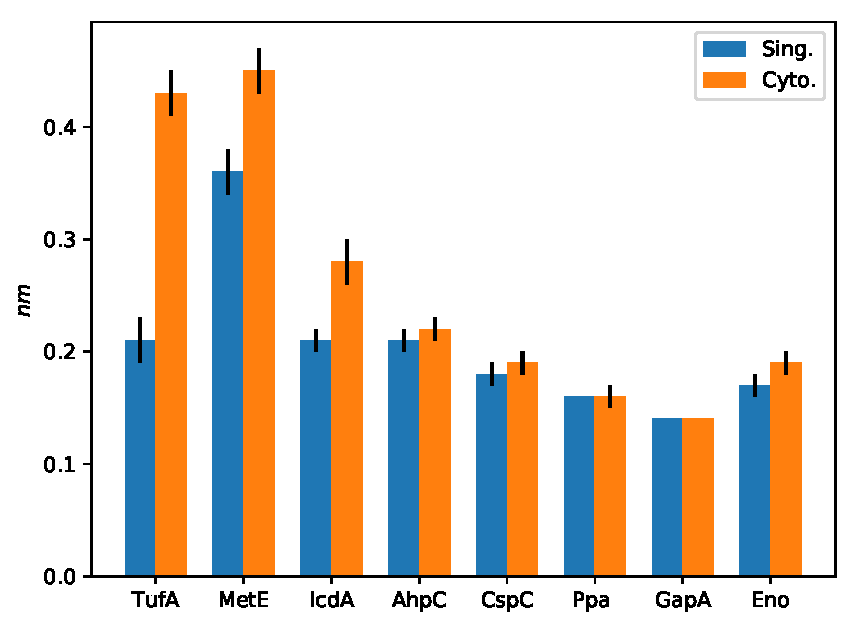
\includegraphics[scale=0.5]{rmsd.pdf}
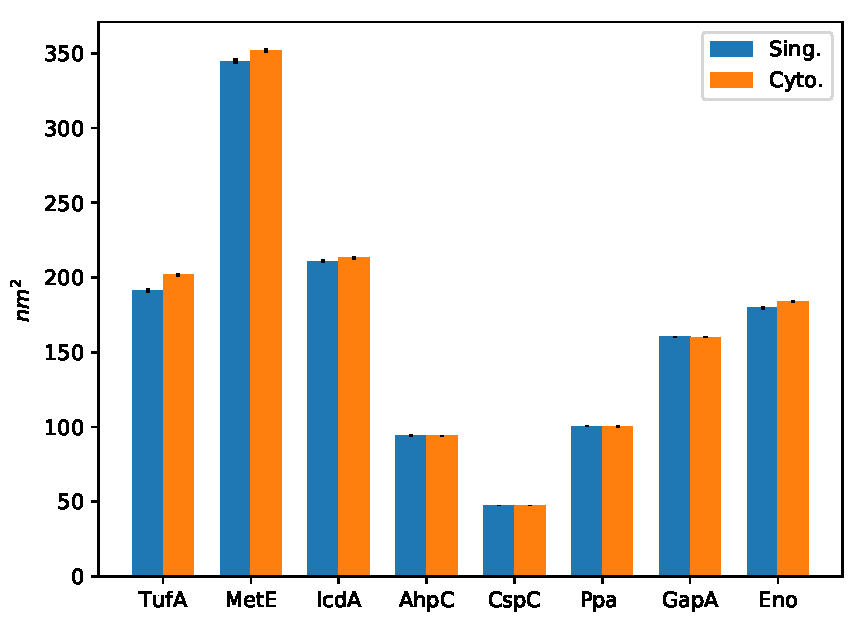
\includegraphics[scale=0.5]{sasa.pdf}

\caption{A) Root mean squared displacement (rmsd) for 8 proteins from single molecule simulation (blue bars) and cytoplasm simulation (orange bars). The average rmsd for each protein in single molecule simulation is over number of chains of proteins and three replica. The average rmsd for each protein in cytoplasm simulation are over number of chains of proteins, number of appearance and three replica. The error bars show the standard errors. B) Chain interface area for oligomers from single molecule simulations (blue bars) and cytoplasm simulations (orange bars). The average value from single molecule simulation is over three replica. The average value from cytoplasm simulation is over the number of proteins and three replica. The error bars show the standard errors. }
\label{fig:structural_integrity_chain}
\end{figure}

% -------------------- STRUCTURAL DYNAMICS --------------------


\subsubsection{Structural dynamics}
Proteins are slightly more flexible in the crowded environment. Root mean square fluctuation (RMSF) calculations show that the flexibility profile of the proteins is not affected by crowding, except in the cases in which there are conformational changes (TufA, MetE and IcdA) (Fig.~\ref{fig:rmsf}). This is in agreement with our results showing that the structural integrity of the proteins is not significantly affected (Fig.~\ref{fig:structural_integrity_chain}A). 
%In addition to that, our results show that the proteins are slightly more flexible in the crowded environment than in the dilute condition. 
This is likely due to the nonspecific interactions that often happen under crowding conditions~\cite{Feig2011, miklos2011, Wang2012b}. The effec of crowded environment on inter-chain interaction of type hydrophobic, hydrogen bonding and salt bridges can be assessed by integrity of oligomeric chains. This is measured as chain interface area (Fig.~\ref{fig:structural_integrity_chain}B). Slightly lower buried area in cytoplasm simulations manifests destabilizing effect of crowded environment on chains of oligomers except except IcdA, GapA and Eno (Fig.~\ref{fig:structural_integrity_chain}B). These three oligomers also show the least changes in their RMSF profiles (Fig.~\ref{fig:rmsf}).


\begin{figure}[H]
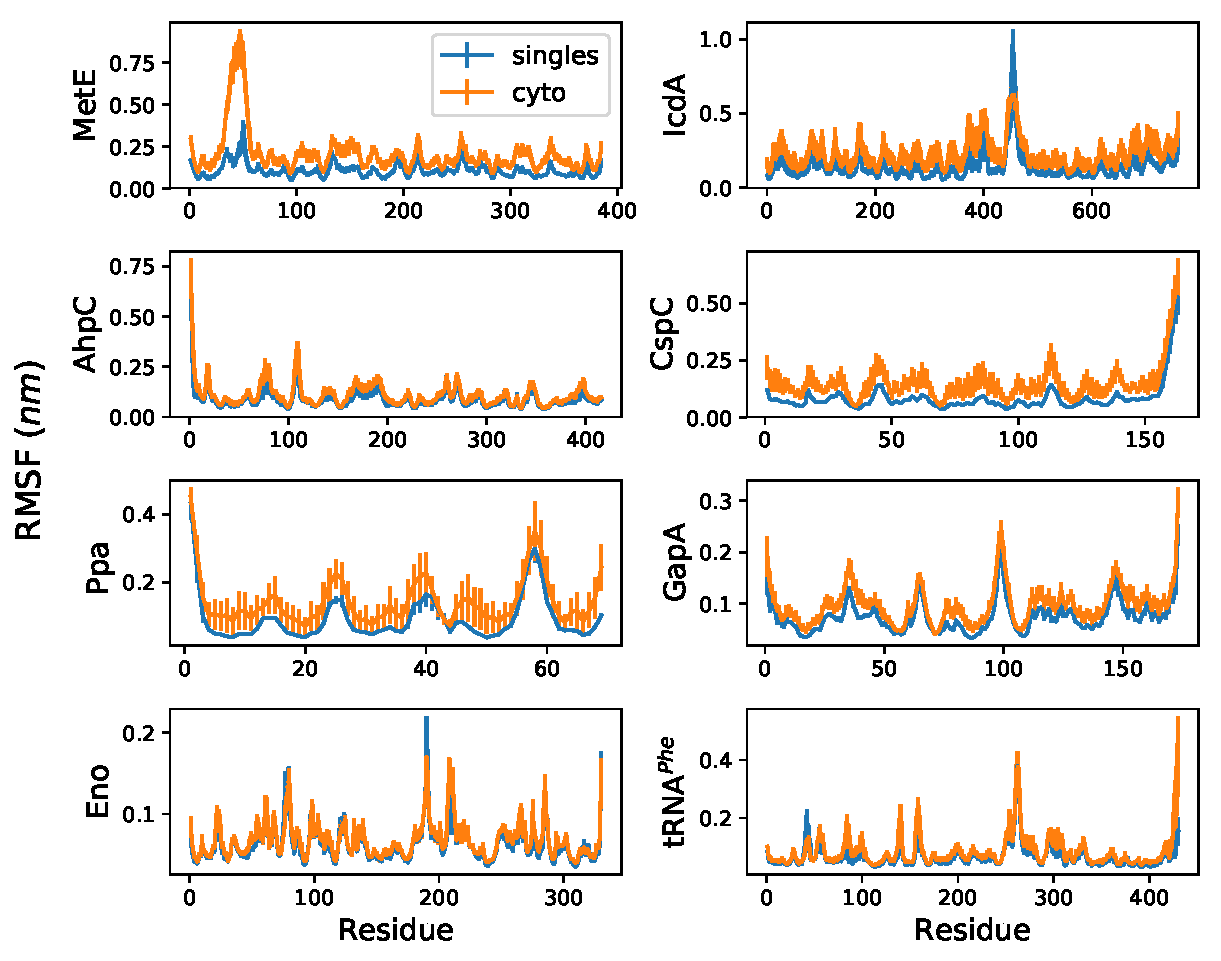
\includegraphics[scale=0.5]{rmsf.pdf}
\caption{Root mean squared fluctuations (rmsf) for 8 crowders from single molecule simulation (blue bars) and cytoplasm simulation (orange bars). x-axis shows the residues for each chain of proteins. The average rmsf for each protein in single molecule simulation is over number of chains of proteins and three replica. The average rmsd for each protein in cytoplasm simulation are over number of chains of proteins, number of appearance and three replica. The error bars show the standard errors.}
\label{fig:rmsf}
\end{figure}





% -------------------- AVOIDING AGGREGATION --------------------

\subsubsection{Aggregation can be avoided by protonating the metabolites}

The initial detection of aggregation in our cytoplasm model was due to the outlier behavior of the translational diffusion constant of tRNA when compared to the other crowders. However, tRNA is not causing such phenomenon (Fig.~\ref{fig:avoiding_aggregation}A). Instead, it is triggered by the exaggerated interaction between the phosphate-containing metabolites, ATP and FBP, with Mg$^{2+}$. tRNA gets involved in the aggregates because Mg$^{2+}$ is present in the box only as counter-ion for ATP and tRNA, and so tRNA is one of the few ``sources'' of Mg$^{2+}$ in the whole system. We looked for ways of avoiding aggregation by simulations of small systems composed of these metabolites in high concentration, Mg$^{2+}$ and water (please check the methods section for details about the parameters we used).

% We found that completely protonating the phosphate groups of ATP and FBP is enough to prevent their aggregation with Mg$^{2+}$ (Fig.~\ref{fig:avoiding_aggregation}B-C). While RDFs show that ATP$^{-3}$ and FBP$^{-4}$ aggregate around Mg$^{2+}$ (Fig.~\ref{fig:avoiding_aggregation}A), this is not observed for ATPH\textsubscript{3} and FBPH\textsubscript{4}(Fig.~\ref{fig:avoiding_aggregation}B-C).

While RDFs show that ATP$^{-3}$ and FBP$^{-4}$ aggregate around Mg$^{2+}$ (Fig.~\ref{fig:avoiding_aggregation}A), we found that completely protonating the phosphate groups of ATP and FBP is enough to prevent their aggregation with Mg$^{2+}$ (Fig.~\ref{fig:avoiding_aggregation}B-C).

\begin{figure}[H]
\hspace*{-2cm}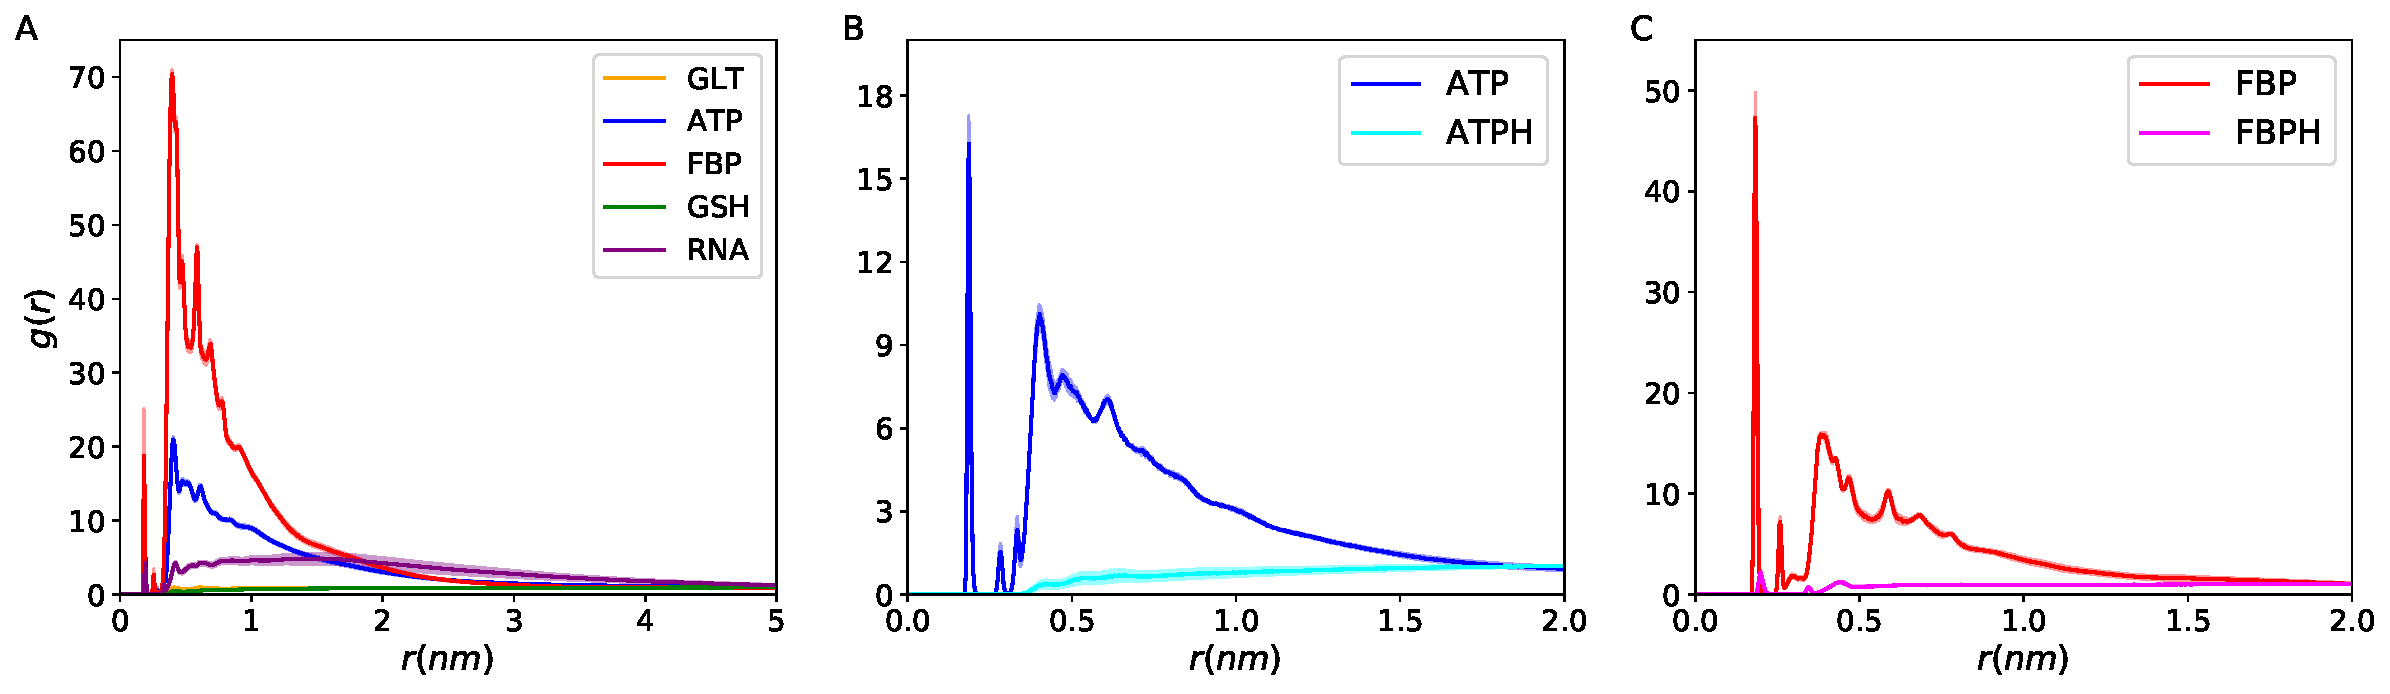
\includegraphics[scale=0.5]{rdf_mg.pdf}
\caption{Radial distribution function (rdf) showing the probability of finding A) metabolites, B) ATP$^{-3}$ or an ATPH\textsubscript{3}, C) FBP$^{-4}$ or an FBPH\textsubscript{4} around MG2+. The averages are over three replica and the shaded regions are the standard errors.}
\label{fig:avoiding_aggregation}
\end{figure}


 
 
 
 
 % -------------------- DISCUSSION --------------------
 
\section*{Discussion}\label{sec:dissc}


The main difference between the behavior of the macromolecules that compose our model in the crowded system and in the dilute condition is their translational diffusion coefficient, which drops by more around 85\% for the proteins and 93\% for the tRNA (Fig.~\ref{fig:translational_diffusion}A). The slope of the line generated by fitting a linear regression model to values of $D_{cyto}/D_{dil}$ is close to zero (slope $= 0.00028$), showing that the drop in diffusion coefficient is independent of the size of the macromolecules. We found that the aggregation of ATP$^{-3}$ and FBP$^{-4}$ around Mg$^{2+}$, which was used as counter-ion for tRNA, leads to its exaggerated confinement. Thus, tRNA is considered as an outlier in our cytoplasm model. In fact, the slope of the linear regression line fitted to $D_{cyto}/D_{dil}$ is reduced by by 50\% and gets even closer to zero (slope $= 0.00014$) after removing the diffusion coefficient of tRNA from the data. Our data is in agreement with experimental results showing that the translational diffusion coefficient of Green Fluorescent Protein (GFP) in {\em E. coli}, as measured by fluorescence recovery after photo-bleaching (FRAP), decreased 90\% when compared to {\em in vitro} measurements~\cite{Elowitz1999,Konopka2006}.


It has been demonstrated that each of the force fields that are most widely used to perform molecular dynamics simulations of macromolecules have different results for highly concentrated amino acid solutions~\cite{andrews2013}. Moreover, it has been reported that simulations of highly concentrated environment leads to aggregation by using additive force fields~\cite{Petrov2014a,Abriata2015a, Nawrocki2017a}. Several solutions has been proposed to eliminate aggregation~\cite{Best2014a,Piana2015a, Bashardanesh2018b}. Previous all-atom simulations of high scale cytoplasm models used parameters from the CHARMM family of force fields~\cite{Yu2016a}, whose solvent-solute interactions are strengthened according to the solution proposed by Best {\em et al.}~\cite{Best2014a}. In this work we use the AMBER force fields~\cite{Best2014a} to study crowding effects on a cytoplasm model. All-atom explicit solvent molecular dynamics simulations have been reported for large-scale cytoplasm models of \textit{Mycoplasma genitalium} composed of 103 and 12 million atoms that were simulated for 20 and 60 \SI{}{\nano\second}, respectively~\cite{Yu2016a}. The cytoplasm model described in this work has 1.5 million atoms and was simulated for the total of \SI{3}{\micro\second}, an unprecedented time scale to study crowding effects on a heterogeneous cytoplasm model in atomic detail.


All crowders are as compact in the cytoplasm model as they are in dilute conditions (Fig.~\ref{fig:structural_integrity_chain}). Despite this overall stability, three crowders (TufA, MetE and IcdA) displayed greater deviation from their crystallographic structure in the cytoplasm model when compared to the dilute condition, indicating that there was some degree of local unfolding (Fig.~\ref{fig:structural_integrity_chain}). Interestingly, the flexibility profiles calculated considering the C$\upalpha$ for each chain of the elements of our cytoplasm model show that, in the crowded condition, most of the proteins (TufA, MetE, AhpC, CspC and Ppa) are slightly more flexible than in the dilute condition (Fig.~\ref{fig:rmsf}). This is in agreement with simulation~\cite{Feig2011} and experiment~\cite{miklos2011,Wang2012b} showing that crowders can destabilize the native structure of proteins due to the numerous unspecific short-lived interactions that are formed between them in a crowded environment.

Having variation of oligomeric state of the crowders in our model (Table~\ref{tbl:protein_fraction}) enabled us to study the effec of crowding on inter-chain interactions. We found out that the oligomers are either slightly destabilized, or no effect is seen (GapA and Eno) (Fig.~\ref{fig:structural_integrity_chain}B). This is in agreement with rmsf results (Fig.~\ref{fig:rmsf}).


Magnesium cations were added to our cytoplasm model as counter-ions for tRNA and ATP. However, as the simulation progressed, FBP and ATP aggregated around Mg$^{2+}$ and, by consequence, around tRNA. After identifying this problem, we used simulations of small systems containing only the metabolites, Mg$^{2+}$ and water to test different strategies to prevent aggregation in future studies using long simulations of cytoplasm models. We found that protonating the phosphate-containing metabolites is enough to reach this goal (Fig.~\ref{fig:avoiding_aggregation}). Even though ATPH$_3$ and FBPH$_4$ are not the biologically relevant forms of these molecules in physiological pH, we consider that using their protonated forms is a good compromise between parametrization complexity and practical results. The biggest impact of this approach is on long range interactions of these metabolites with other molecules due to the neutralization of their net charge. However, molecules in a crowded environment are restrained to smaller volumes and shorter inter molecular distances, which mitigates the effect of charge neutralization.

To the best of our knowledge, there is only one work in the literature which studied large scale cytoplasm models that included metabolites with all-atom explicit solvent molecular dynamics~\cite{Yu2016a}. Although they didn't report aggregation, they mentioned that the translational diffusion of highly charged phosphate-containing metabolites was ``much slower'' than expected. They attributed this observation to non-specific interactions between such metabolites and proteins. Maybe aggregation also contributed to their slower diffusion but it was not evident during \SI{140}{\nano\second}, which was the length of their longest simulation.


 
 
% -------------------- CONCLUSIONS --------------------

\section*{Conclusions}\label{sec:concl}

In this work we built a cytoplasm model...


the model was validated by reproducing experimental data about the reduction of the translational diffusion coefficient of proteins in E.coli.

the model is stable.

however, aggregation!

In the specific case of ATP and FBP modeled with GAFF in boxes containing Mg$^{2+}$, we advise that they should be completely protonated even though that is not their physiological protonation state. The topology and structure files we are providing for ATP and FBP on github are already protonated.

In principle it is possible to develop new parameters for phosphate and Mg that doesn't lead to aggregation. However this is outside of the scope of this study and 
 
\bibliography{library}

% \begin{addendum}
%  \item  
%  \item[Competing Interests] 
%  \item[Correspondence]  
% \end{addendum}
 
\end{document}


